%-------------------------------------------------------------------------------
\section{Preliminary Results}
%-------------------------------------------------------------------------------

In order to provide some evidence that \sys{}'s design meets its goals,
this section answers two questions: (1) does \sys avoid the \problem?
(\autoref{s:hermod}) and (2) is swapping a feasible approach to
managing memory of functions? (\autoref{s:memory})

\begin{figure}[t!]
    \centering
      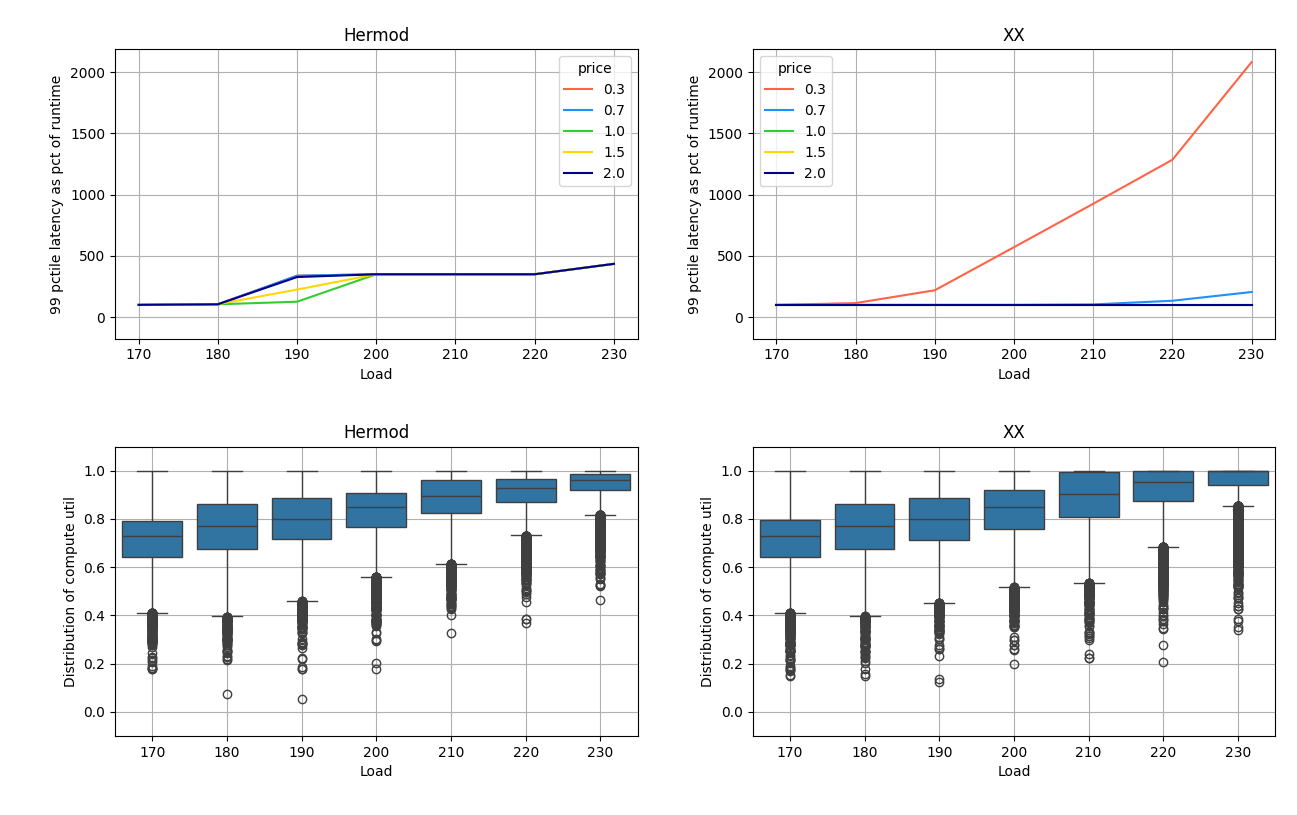
\includegraphics[width=8.5cm]{img/hermod_xx_latencies.png}
      \caption{ tail latency distribution for Hermod and \sys{}, for high (top)
      and low (bottom) \priceclass{} functions. At tick 50 (first red line) the
      load was increased, and at tick 80 (second red line) it was decreased again
      }
    \label{fig:hermod-xx-latencies}
\end{figure}


\subsection{Experimental methodology}

To answer these questions, we build a simulator in Go\cite{golang} in
which functions arrive in an open loop. The simulator attaches three
properties to each function: runtime, \priceclass{}, and memory
usage.~\textit{Function runtime} is chosen by sampling from randomly
generated long tailed (pareto) distribution: the length of the tail
($\alpha$ value) is constant, and the minimum value ($x_m$) is chosen
from a normal distribution. This sampling reflects the fact that
different functions have different expected runtimes (represented by
$x_m$), and that actual invocation runtimes follow long tailed
distributions (represented by the pareto function).~\textit{Function
  \class{}} is chosen randomly, but weighted: the simulator uses a
bimodal weighting across $n$ \priceclass{} values, each assigned to a
fictitious price. Because functions are randomly assigned a \class{},
runtime and \class{} are not correlated.~\textit{Function memory
  usage} is chosen randomly between 100MB and 10GB. Over their
lifetime, functions increase their memory usage from an initial amount
(always 100MB) to their total usage.

The simulator makes a few simplifying assumptions: (1) functions are
compute bound, and do not block for I/O; and (2) communication and
swap latencies are not simulated.

We simulate running 100 machines with 8 cores each, 4 scheduler
shards, and run $k=3$ for $k$-choices.

\subsection{Does \sys{} avoid the \problem{}?}
\label{s:hermod}
  
To show that \sys{} can run high-classes functions quickly even under
high load, we compare \sys{} with Hermod, a state-of-the-art research
scheduler built specifically for serverles~\cite{hermod}. We simulate
Hermod in the best configuration according to the paper: least-loaded
load balancing over machines found using power-of-$k$-choices,
combined with early binding and Processor Sharing machine-level
scheduling. Because Hermod does not account for memory limits on
machines, we ignore memory in this experiment.  We also turn off the
use of the idle list in \sys{}, so as to be on par with Hermod in
placing load.

We run an experiment that starts with a medium load setting,
temporarily increase the load, and then return to the baseline load. A
strong result for \sys{} would show that it is able to maintain low
latency for high \priceclass{} functions, even under the high load.
Figure~\ref{fig:hermod-xx-latencies} shows the results. We can see
that \sys{} is indeed able to maintain low latencies for the high
\class{} functions, at the cost of increasing the latencies for low
\class{} functions. Hermod spreads the performance degradation across
all the different functions equally.

\subsection{Is swapping memory of functions feasible?}
\label{s:memory}
  
\begin{figure}[t!]
    \centering
      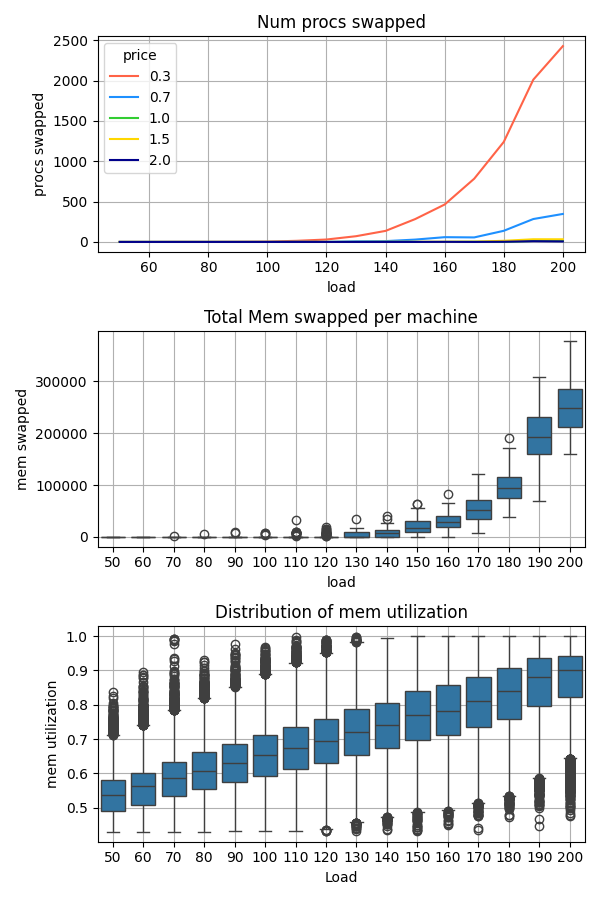
\includegraphics[width=8cm]{img/memory_graphs.png}
      \caption{ \sys{}'s swapping behavior. The amount of memory is in MB  }
    \label{fig:memory-graphs}
\end{figure}

To answer this question, we count the amount of swap memory that \sys{}
uses and which functions \sys{} swaps. We configure the simulator to run \sys{}
with limited memory (32GB of RAM per machine). A good result would
show: a small spread of memory utilization, that machines start
swapping only once memory utilization is high, that the amount of
swapping being done is equally spread across machines, and that
high-class functions are not impacted by
swapping. Figure~\ref{fig:memory-graphs} shows the results. We can see
\sys{} swaps only lower \class{} functions' memory, and that the
amount of memory swapped is fairly evenly distributed between all the
machines. We can also conclude that with a 500GB~SSD, a provider would
be able to avoid killing while running the datacenter at an average
memory utilization of $\sim$90$\%$, at the cost of $\sim\$$30 per
machine for swap space~\cite{ssd-price}.


